Последовательность графов, у которых $\rho^{max}$ стремится к иррациональному числу, можно использовать для доказательства отсутствия закона нуля или единицы при рациональных $\alpha$.

Рассмотрим граф, изображённый на Рис.~\ref{fig:first block}.
\begin{figure}[h]
  \centering
  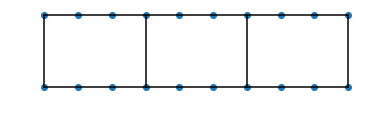
\includegraphics[scale=0.5]{picrel/first_block.png}
  \caption{Первый блок}
  \label{fig:first block}
\end{figure}

Если присоединить к нему кусочек, как на рисунке \ref{fig:2 blocks}, то плотность и максимальная плотность графа не изменятся

\begin{figure}[h]
  \centering
  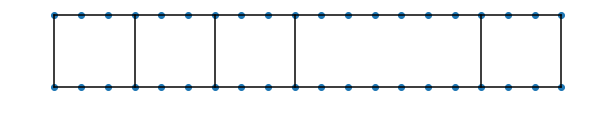
\includegraphics[scale=0.5]{picrel/2_blocks.png}
  \caption{Два блока}
  \label{fig:2 blocks}
\end{figure}

Можно присоединить 9 кусочков, увеличив число рёбер и 
вершин в десять раз, затем добавить (или не добавлять) одно ребро. Получившийся граф будет иметь вид, как граф на рисунке \ref{fig:additional edge}

Таким образом можно увеличивать число рёбер и вершин в $10^k$ раз и добавлять ребро.
Последовательность плотностей графов будет стремиться к бесконечной апериодической десятичной дроби.

\begin{figure}[ht]
  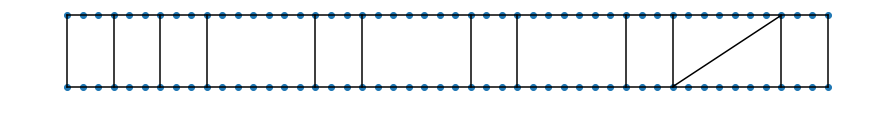
\includegraphics[scale=0.5]{picrel/additional_edge.png}
  \caption{Несколько блоков и дополнительное ребро}
  \label{fig:additional edge}
\end{figure}

Граф состоит из примыкающих друг к другу секций, поэтому для записи формулы, выражающей существование этого или более плотного графа, достаточно столько переменных, сколько нужно, чтобы выразить существование наибольшей из секций. 